\def\thetitle{Homework 1}
\pagebreak

\begin{center}
    
\includegraphics[height=0.075\textheight]{images/LogoYachay.pdf} 
    \hspace{0.1\linewidth}
    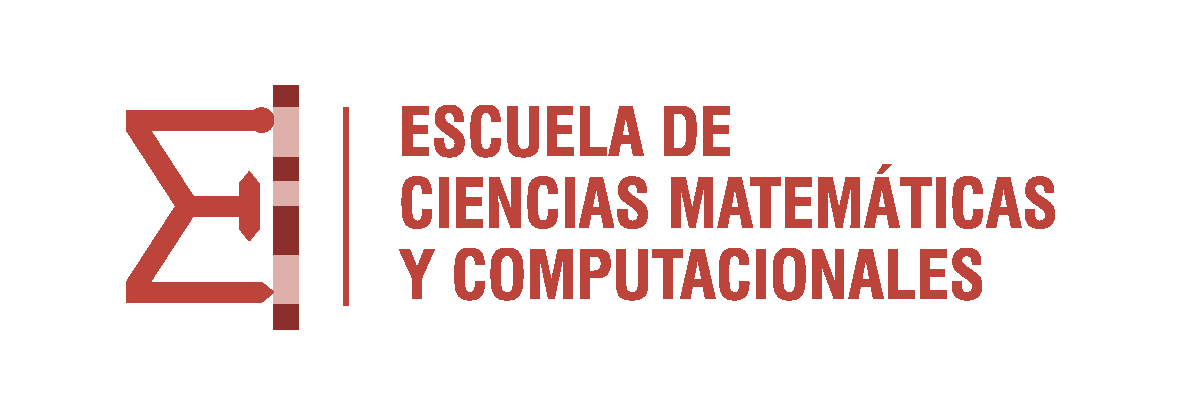
\includegraphics[height=0.075\textheight]{images/LogoECMC.pdf}
\end{center}

% \phantomsection\pdfbookmark{\currfilebase}{\currfilebase}

\begin{center}
    {\LARGE
    Abstract Algebra 2024--I\\
    % Teaching Assistant
    \vspace{0.25cm}
    \textbf{\thetitle{}}}

    % \emph{I hear, I forget;    I see, I remember;     I do, I understand.}
    
    Pablo Rosero \& Christian Chávez
    
    % \today

    September 11, 2023
\end{center}

% \setcounter{problem}{0}


\begin{questions}

\question
  For each of the following pairs of integers \(a\) and \(b\), determine their greatest common divisor, their least common multiple, and write their greatest common divisor in the form \(a x+b y\) for some integers \(x\) and \(y\).
  \begin{enumerate}[label=(\alph*)]
    \item \(a=792, b=275\)
    \item \(a=507885, b=60808\)
  \end{enumerate} 

\begin{solution} Using the (extended) Euclidean Algorithm, we get the following. Here \([a,b]\) denotes the least common multiple of \(a\) and \(b\).
    \begin{enumerate}[label=(\alph*)]
        \item \((a,b) = 11\), \([a,b] = 19800\), \((a,b)= 8a - 23b\)
        \item \((a,b) = 691\), \([a,b] = 44693880\), \((a,b)= -17a +142b\)
    \end{enumerate}
\end{solution}


\question
    Prove that if \({n}\) is composite then there are integers \(a\) and \(b\) such that \(n\) divides \(a b\) but \(n\) does not divide either \(a\) or \(b\).

\begin{theproof}
    Let \(n\) be composite. Recall this means \(n\) is a positive integer greater than \(1\). By definition, \(n\) has positive divisors other than \(1\) and \(n\). Thus, \(n=a b\) for some positive integers \(a\) and \(b\) with \(a,b\notin \left\{ 1,n \right\}\). Clearly \(n \mid a b\).
    Since \(a < n\), we have \(n\nmid a\). Similarly \(n\nmid b\). We are done.
    % Now suppose by way of contradiction that \(n \mid a\). Then we have \(k n=a\) for some integer \(k\). Now \(k b a=a\), so \((k b-1) a=0\), so \(k b=1\). Thus \(b= \pm 1\), a contradiction. Hence,  \(n\) does not divide \(a\). Similarly, \(n\) does not divide \(b\).
\end{theproof}

\question
    If \(p\) is a prime, prove that there do not exist nonzero integers \(a\) and \(b\) such that \(a^2=p b^2\). (Why this proves  \(\sqrt{p}\) is not a rational number.)
\renewcommand{\solutiontitle}{}
    \begin{solution}%[-10cm]
    \vspace*{-\baselineskip}
    % Let's use basic facts from the integers. 
    \begin{proof}
    Suppose \(p\) is a prime number and assume for the sake of contradiction that there do exist nonzero integers \(a\) and \(b\) such that \(a^2=p b^2\).
    Either \(a\) and \(b\) share common factors other than \(1\) or not.
%
    Suppose first they do not have commont factors other than \(1\).
    Notice \(a^2=p b^2\) implies \(p\mid a^2\), whence \(p\mid a\) (by Euclid's lemma), and thus  \(pk = a\) for some \(k\in \Z\). Thus, \(p^2k^2 = p b^2\) which implies \(p k^2 = b^2\). Then,  \(p\mid b^2\) and, as before,  \(p\mid b\). We have shown \(p\) divides both \(a\) and \(b\), so \(p\) is a common factor of both, a contradiction.
%
    If \(a\) and \(b\) share common factors other than \(1\), we can rule them out of the equation \(a^2=p b^2\) by using the Fundamental Theorem of Arithhmetic to write \(a^2\) and \(b^2\) as powers of products of primes. Hence, we are led to the case above, which we proved cannot hold. 
%
    In any case we arrived at a contradiction and so we conclude our main assumption was false. The proof is complete.
    \end{proof}

    \textbf{Remark.} Euclid's lemma states that if a prime number divides the product of two integers, then it must divide at least one of those integers. On the other hand, this proof uses basic facts about the integers. However, by writing \((a/b)^2 = p\), with \(a\) and \(b\) in lowest terms, we see that \(b=1\) because \(p\) is an integer and the rationals that are also integers are the ones that have denominator \(1\). Thus \(a^2 = p\) implies \(p\) is composite, a contradiction.
\end{solution}
\renewcommand{\solutiontitle}{\noindent\textit{Solution.} }

% Dummit p. 11 ------------------------

\question
    Write down explicitly all the elements in the residue classes of \(\mathbb{Z} / 18 \mathbb{Z}\).
\begin{solution} The elements of \(\mathbb{Z} / 18 \mathbb{Z}\) are 
    $$\begin{gathered}
        \{18 k \mid k \in \mathbb{Z}\},\{1+18 k \mid k \in \mathbb{Z}\},\{2+18 k \mid k \in \mathbb{Z}\} \\
        \{3+18 k \mid k \in \mathbb{Z}\},\{4+18 k \mid k \in \mathbb{Z}\},\{5+18 k \mid k \in \mathbb{Z}\} \\
        \{6+18 k \mid k \in \mathbb{Z}\},\{7+18 k \mid k \in \mathbb{Z}\},\{8+18 k \mid k \in \mathbb{Z}\} \\
        \{9+18 k \mid k \in \mathbb{Z}\},\{10+18 k \mid k \in \mathbb{Z}\},\{11+18 k \mid k \in \mathbb{Z}\} \\
        \{12+18 k \mid k \in \mathbb{Z}\},\{13+18 k \mid k \in \mathbb{Z}\},\{14+18 k \mid k \in \mathbb{Z}\} \\
        \{15+18 k \mid k \in \mathbb{Z}\},\{16+18 k \mid k \in \mathbb{Z}\},\text{ and }\{17+18 k \mid k \in \mathbb{Z}\}.
        \end{gathered}$$
    Note however that a more compact way to write this information is as follows: \[
        \Z/18\Z = \bigcup_{i=0}^{17} \left\{ \{i+18k \mid k\in \Z\} \right\}.
    \]
\end{solution}

\question
    Suppose \(a=a_n 10^n+a_{n-1} 10^{n-1}+\cdots+a_1 10+a_0\) is any positive integer. Show  that \(a \equiv a_n+a_{n-1}+\cdots+a_1+a_0\pmod 9\). (Note that this is the usual arithmetic rule that the remainder after division by 9 is the same as the sum of the decimal digits mod \(9\). In particular, an integer is divisible by 9 if and only if the sum of its digits is divisible by 9).
    %[note that \(10 \equiv 1(\bmod 9)\) ].
\begin{theproof}
    Let \(\overline{a}\) denote the residue class of \(a\) mod \(9\). Using modular arithmetic we have 
    \[
        \overline{a}=\overline{\sum_{k=0}^n a_{k} 10^k}=\sum_{k=0}^n{\overline{a_k}}\cdot \overline{10}^k=\sum_{k=0}^n \overline{a_k} \cdot 1.
    \] 
    Equivalently, this can be written as 
    \[a \equiv a_n+a_{n-1}+\cdots+a_1+a_0\pmod 9,\]
    and we are done.
\end{theproof}

\question
    Compute the remainder when \(37^{100}\) is divided by 29.

\begin{solution}
    Performing all arithmetic mod \(29\), we have \(37^{100}=8^{100}\). Moreover, note that
\[
\begin{aligned}
8^{28} & =\left(8^2\right)^2 \cdot\left(\left(8^2\right)^2\right)^2 \cdot\left(\left(\left(8^2\right)^2\right)^2\right)^2 \\
& =6^2 \cdot\left(6^2\right)^2 \cdot\left(\left(6^2\right)^2\right)^2 \\
& =7 \cdot 7^2 \cdot\left(7^2\right)^2 \\
& =7 \cdot 20 \cdot 20^2 \\
& =140 \cdot 23 \\
& =24 \cdot 23 \\
& =552 \\
& =1 .
\end{aligned}
\]

So we have \(8^{100}=8^{28} \cdot 8^{28} \cdot 8^{28} \cdot 8^{16}=8^{16}=23\), as computed above.
\end{solution}

\question
    Prove that the squares of the elements in \(\mathbb{Z} / 4 \mathbb{Z}\) are just \(\overline{0}\) and \(\overline{1}\).
\begin{theproof}
    We have \(\mathbb{Z} / 4 \mathbb{Z} =\left\{ \overline{0},\overline{1},\overline{2},\overline{3} \right\}  \). 
    Modulo 4, we have \(\overline{0}^2 = \overline{0}\), \(\overline{1}^2 = \overline{1}\), \(\overline{2}^2 = \overline{4} = \overline{0}\), and \(\overline{3}^2 = \overline{9} = \overline{1}\).
    %  { Modulo } 4 \text {, we have } \overline{0}^2=\overline{0},, \overline{2}^2=\overline{4}=\overline{0} \text {, and } \overline{3}^2=\overline{9}=\overline{1}.
\end{theproof}

\question
    Let \(a,b\in \Z\).
    Prove  that \(a^2+b^2\) never leaves a remainder of 3 when divided by 4. (Hint: use the previous exercise.)
\begin{theproof}
    Suppose \(a^2+b^2\) can be divided by \(4\) (so, it is not zero). 
    By the division algorithm, there are unique integers \(q\) and \(r\) such that \(a^2+b^2 = 4q +r\) with \(0\leq r < 4\). Then \(\overline{a^2+b^2} \equiv \overline{r}\), taking congruence classes mod \(4\). By the previous exercise, \(\overline{a^2+b^2}=\overline{a}^2 + \overline{b}^2\) can only be \(\overline{0}\), \(\overline{1}\) or \(\overline{2}\). Thus \(\overline{r}\neq \overline{3}\), whence \(r\neq 3\). 
\end{theproof}


\question
    Prove that the equation \(x^2+y^2=3 z^2\) has no solutions for \(x,y,z\in\Z\).
    %(Consider the equation mod 4 as in the previous two exercises and show that \(a, y\) and \(z\) would all have to be divisible by 2. Then each of \(x^2\), \(y^2\) and \(c^2\) has a factor of 4 and by dividing through by 4 show that there would be a smaller set of solutions to the original equation. Iterate to reach a contradiction.)
\begin{theproof}%(The hint is the sketch of one proof. Here  is an alternative.)
    Suppose, to the contrary, there are  are nonzero integers  \(x\), \(y\), and \(z\) such that \(x^2 + y^2 = 3 z^2\).
    Either these integers have  factors in common or not.
    %    
    If they do, we can factor them out of the equation \(x^2 + y^2 = 3 z^2\) to get a new equation \(\hat{x}^2 + \hat{y}^2 = 3 \hat{z}^2\) where \(\hat{x}\), \(\hat{y}\) and \(\hat{z}\) do not share common factors. This situation lead us to the second case, so we only need to prove such a case is imposible.
    Suppose  \(x\), \(y\), and \(z\) do not share common factors.
    Taking residue classes modulo \(3\), we have \(\overline{x}^2 + \overline{y}^2 = \overline{0}\). This equation is satisfied (if and) only if \(x\) and \(y\) are multiples of \(3\).
    Indeed, if \(k\) is any integer, then \(\overline{k}\) can only be \(\overline{0}\), \(\overline{1}\) or \(\overline{2}\); thus \(\overline{k}^2\) can only be \(\overline{0}\) or \(\overline{1}\). Since \(\overline{1} + \overline{0} = \overline{0} + \overline{1} = \overline{1}\) and \(\overline{1} + \overline{1} = \overline{2}\), the only possible case is \(\overline{x}^2 = \overline{y}^2 = \overline{0}\).
    In other words, \(3\mid x^2\) and \(3\mid y^2\).
    Euclid's lemma then implies \(3\) divides both \(x\) and \(y\). Finally, it follows the left side of \({x}^2 + {y}^2 = 3 {z}^2\) is a multiple of \(9\) and by dividing both sides by \(3\) we get \(z^2\) is a multiple of \(3\), whence \(z\) is also a multiple of \(3\). We have shown that \(x\), \(y\), and \(z\) have  \(3\) as common factor, which is a contradiction. 
    This contradiction proves the result.
\end{theproof}


\question
    Prove that if \(\overline{a}, \overline{b} \in(\mathbb{Z} / n \mathbb{Z})^{\times}\), then \(\overline{a} \cdot \overline{b} \in(\mathbb{Z} / n \mathbb{Z})^{\times}\).
\begin{theproof}
    Suppose \(\overline{a}, \overline{b} \in(\mathbb{Z} / n \mathbb{Z})^{\times}\). Then there are \(\overline{x}, \overline{y} \in(\mathbb{Z} / n \mathbb{Z})^{\times}\) such that \(\overline{a}\cdot \overline{x} = \overline{1}\) and \(\overline{b}\cdot \overline{y} = \overline{1}\). Thus \[(\overline{a}\cdot\overline{b})\cdot (\overline{x}\cdot \overline{y}) = (\overline{a}\cdot \overline{x})\cdot (\overline{b}\cdot \overline{y}) = \overline{1},\]
    whence the result follows.
\end{theproof}


\question\label{q.znz.inverses.1}
    Let \(n \in \mathbb{Z}\), \(n>1\), and let \(a \in \mathbb{Z}\) with \(1 \leq a \leq n\). Prove if \(a\) and \(n\) are not relatively prime, there exists an integer \(b\) with \(1 \leq b<n\) such that \(a b \equiv 0\pmod n\) and deduce that there cannot be an integer \(c\) such that \(a c \equiv 1\pmod n\).
\begin{theproof}
    Suppose \(d=(a,n ) > 1\).
    % Recall \(dl = an\) where \(l=[a,b]\).
    % Notice that if \(a=1\), then \(d=1\) which cannot hold. Thus assume \(a>1\).
    % Either \(n\) is a multiple of \(a\) or not. 
    % If it is, then \(ak = n\) for some  \(k\in \Z\) with \(1\leq k < n\)  (note \(k\neq n\) as \(a>1\)). In this case, we take \(b=k\) and we are done.
    % Now suppose \(n\) is not a multiple of \(a\). There are integers \(x\) and \(y\) such that \(ax + ny = d\). Notice here \(y\neq 0\); otherwise \(a\mid d\), and since \(d\mid n\) we would have \(a\mid n\), a contradiction.
    % Recall \(dl = an\) where \(l=[a,b]\).
    % Then \(axl + nyl = dl = an\), whence \(axl \equiv 0\pmod n\).
    By definition, \( a = dx \) and \(dy = n\) for some positive integers \(x\)  and \(y\).
    Thus \(ay = dxy = nx\), whence \(ay \equiv 0\pmod n\). Since \(d >1\), we have \(y < n\). 
    Take \(b = y\).
    If there were an integer \(c\) such that \(a c \equiv 1\pmod n\), then \(abc \equiv b \pmod n\), whence \(0\equiv b\pmod n\). This is a contradiction since \(1 \leq b<n\).
\end{theproof}


\question\label{q.znz.inverses.2}
    Let \(n \in \mathbb{Z}\), \(n>1\), and let \(a \in \mathbb{Z}\) with \(1 \leq a \leq n\). Prove that if \(a\) and \(n\) are relatively prime then there is an integer \(c\) such that \(a c \equiv 1\pmod n\). (Use the fact that the g.c.d. of two integers is a \(\mathbb{Z}\)-linear combination of the integers.)
\begin{theproof}
    Suppose \(a\) and \(n\) are relatively prime. We know there are integers \(x\) and \(y\) such that \(ax+ny = (a,b) = 1\). Thus \(ax \equiv  1\pmod n\). Take \(c=x\) and conclude.
\end{theproof}


\question
    Conclude from the previous two exercises that \((\mathbb{Z} / n \mathbb{Z})^{\times}\)is the set of elements \(\bar{a}\) of \(\mathbb{Z} / n \mathbb{Z}\) with \((a, n)=1\) and hence prove Proposition 4 . Verify this directly in the case \(n=12\).
\begin{solution}
From \ref{q.znz.inverses.1},  it follows  \((\mathbb{Z} / n \mathbb{Z})^{\times}\subseteq \left\{ \overline{k}\in\mathbb{Z} / n \mathbb{Z} : (k,n) = 1 \right\}\)  (use the contrapositive). From \ref{q.znz.inverses.2}, it follows the other inclusion and consequently \[(\mathbb{Z} / n \mathbb{Z})^{\times}= \left\{ \overline{k}\in\mathbb{Z} / n \mathbb{Z} : (k,n) = 1 \right\}.\]
In particular, \[
    (\mathbb{Z} / 12 \mathbb{Z})^{\times}=
    \left\{ 
        1,5,7,11
     \right\}.
\] The inverses of these elements are \(1\), \(5\), \(7\), and \(11\), in display order.
\end{solution}


% Page 51 from [Rotman 2006] ----------------------------------

\question
    \begin{enumerate}[label=(\alph*)]
        \item Prove that if \(n\) is squarefree (i.e., \(n>1\) and \(n\) is not divisible by the square of any prime), then \(\sqrt{n}\) is irrational.
        \item Prove that \(\sqrt[3]{2}\) is irrational.
    \end{enumerate}


\begin{theproof}
\begin{enumerate}[label=(\alph*)]
    \item Suppose \(n\) is square free  and assume, for the sake of contradiction, that \(\sqrt{n}\) is rational.
    Thus, \(\sqrt{n}= p/q\) for some integers \(p\) and \(q\) with \((p,q)=1\).
    Then \(n = p^2 / q^2\), and since \((p^2, q^2) = 1\) (verify this by using the procedure to compute the g.c.d. using the FTA), it follows \(q^2 = 1\) because \(n\) is an integer (a rational number with denominator \(1\)). 
    Thus, \(n= p^2\). Note \(n>1\) implies \(p\) can be written as a product of powers of primes. 
    Then \(p^2\) contains the square of a prime in its prime factorization. Since the square of a prime divides \(p^2=n\), we reach a contradiction. The proof is finished.

    \item We know \(2\) is square free. Thus \(\sqrt{2}\) is irrational. It follows \(\sqrt[3]{2}\) is irrational. Otherwise we could write \(\sqrt[3]{2}\) as a quotient of integers and from there it is implied \(\sqrt{2}\) is a rational number, by the properties of exponentiation. Contradiction.
\end{enumerate}
\end{theproof}


\question
Let \(a\) and \(b\) be nonzero integers and let \(d=(a, b)\). Prove that \(a / d\) and \(b / d\) are relatively prime.
\begin{theproof}
    There are integers \(x\) and \(y\) such that \( ax+ by = d\), so
    \[\frac{a}{d}x + \frac{b}{d}y = 1.\] 
    Let \(d' = (a/d, b/d)\).
    Because \(d'\) divides any \(\Z\)-linear combination of \(a/d\) and \(b/d\), it follows \(d'\mid 1\). 
    Hence \(d'=1\) and the proof is complete.
\end{theproof}


\question
    Let \(m,r,r'\in\Z\).
    Prove that if \((r, m)=1=\left(r^{\prime}, m\right)\), then \(\left(r r^{\prime}, m\right)=1\).
\begin{theproof}
    Suppose \((r, m)=1=\left(r^{\prime}, m\right)\). Then \(rx_1 + my_1 =1\) and \(r'x_2 + my_2 =1\) for some integers \(x_1,x_2,y_1,y_2\). Thus
    \begin{align*}
         (rx_1 + my_1)r'x_2 + (rx_1 + my_1)my_2 &=1\\
    \iff rr'x_1x_2 + m(y_1r'x_2 + rx_1y_2 + my_1y_2)   & = 1.
    \end{align*}
    Since \(\left(r r^{\prime}, m\right)\) divides any \(\Z\)-linear combination of \(rr'\) and \(m\), it follows \(\left(r r^{\prime}, m\right)\mid 1\) and thus \(\left(r r^{\prime}, m\right) = 1\), as desired.
\end{theproof}


\question
    Assume that \(d=s a+t b\) is a \(\Z\)-linear combination of integers \(a\) and \(b\).
    Find infinitely many pairs of integers \(\left(s_k, t_k\right)\) with \(d=s_k a+t_k b\).
\begin{solution}
    For every \(k\in \Z\), let  \(s_k = s-kb\) and \(t_k = t + ka\). Notice   \[
        s_k a + t_k b = sa - kab + tb + kab = sa + tb = d
    \] for every \(k\in \Z\). Thus, there are countably many pair of integers \(\left( s_k, t_k \right)\) that satisfy the equation. We are done.
\end{solution}


\question
    If \(a\) and \(b\) are relatively prime and if each divides an integer \(n\), then their product \(a b\) also divides \(n\).
\begin{theproof}
    Suppose \(a\) and \(b\) are relatively prime and that each one divides an integer \(n\).
    Let \(d= \left( a,b \right)\) and \(l=[a,b]\).
    Since \(n\) is  a common multiple of \(a\) and \(b\), we must have \(l\mid n\).
    Notice \(l=ab\) because   \(dl = ab\) and  \(d=1\). Thus \(ab\mid n\), as desired.
\end{theproof}


\question
Let \(a,b,c\in\Z\) with  \(a>0\). Prove that \(a(b, c)=(a b, a c)\). (One must assume that \(a>0\) lest \(a(b, c)\) be negative.)
\begin{theproof}
    Write \(bx+cy = (b,c)\) for some integers \(x\) and \(y\). Then  \(abx+acy = a(b,c)\). Since \((a b, a c)\) divides any \(\Z\)-linear combination of \(ab\) and  \(ac\), it follows \((a b, a c)\mid a(b,c)\). 
    On the other hand, note \(a(b,c)\mid ab\) and \(a(b,c)\mid ac\), so \(a(b,c)\) divides any \(\Z\)-linear combination of \(ab\) and \(ac\). In particular, \(a(b,c)\mid (ab,ac)\).
    Therefore, because \(a(b,c)\) and \((ab,ac)\) divide each other and they are positive, it follows \(a(b, c)=(a b, a c)\).
\end{theproof}


\question
     A Pythagorean triple is a 3-tuple \((a, b, c)\) of positive integers for which
\[
a^2+b^2=c^2.
\] A pythagorean triple is  called primitive if  \(\operatorname{gcd}(a, b, c)=1\). (\textit{Definition.} A common divisor of nonzero integers \(a_1, a_2, \ldots, a_n\) is an integer \(c\) such that \(c \mid a_i\) for all \(i\in \left\{ 1,\dots,n \right\}\). The largest of the common divisors   is called its greatest common divisor.)
\begin{enumerate}[label=(\alph*)]
    \item Consider a complex number \(z=q+i p\), where \(q>p\) are positive integers. Prove that
\[
\left(q^2-p^2, 2 q p, q^2+p^2\right)
\]
is a Pythagorean triple by showing that \(\left|z^2\right|=|z|^2\). (One can prove that every primitive Pythagorean triple \((a, b, c)\) is of this type.)
\item Show that the Pythagorean triple \((9,12,15)\) (which is not primitive) is not of the type given in part (a).

\end{enumerate}
\begin{theproof}
\begin{enumerate}[label=(\alph*)]
    \item Note \(|z^2| = |z\cdot z| = |z||z|=|z|^2\).
    Now \(z^2=\left(q^2-p^2\right)+i 2 q p\), so that \(\left|z^2\right|=\left(q^2-p^2\right)^2+(2 q p)^2\). On the other hand, \(|z|^2=\left(q^2+p^2\right)^2\). Thus, if we define \(a=q^2-p^2\), \(b=2 q p\), and \(c=q^2+p^2\), then \(a^2+b^2=c^2\). We have shown  \((a, b, c)\) is a Pythagorean triple, completing the proof.

    \item Suppose there are positive integers \(p\) and \(q\), with \(q>p\), such that  \((9,12,15)\) is a pythagorean triple of the type above. Then \(2 q p=\) 12 and \(q p=6\). Since \(q>p\) are positive integers, the only possibilities are \(q=6\) and \(p=1\) or \(q=3\) and \(p=2\). The first possibility gives the Pythagorean triple \((12,35,37)\) while the second gives the Pythagorean triple \((5,12,13)\).  Contradiction.
\end{enumerate}
\end{theproof}


\question
    Let \(X\) and \(Y\) be finite sets. Show that there is a bijection \(f\colon X \rightarrow Y\) if and only if \(|X|=|Y|\). (By definition, a set is finite if it is empty or if it can be put in a one-to-one correspondence with \([k] = \left\{ 1,2,\ldots, k \right\}\), for some integer \(k\geq 1\).)

\begin{proof} There is nothing to prove. This is the definition of cardinality. 
    % See Rotman, p. 94.
% \begin{itemize}
%     \item[(\(\Rightarrow\))] If \(f\colon X \rightarrow Y\)  is a bijection, it follows, by definition, that \(|X|=|Y|\).
%     \item[(\(\Leftarrow\))]  Suppose \(m=n\). Since \(X\) is finite, it can be put in a one-to-one correspondence with \([m]\). Similarly, \(Y\) can be put in a one-to-one correspondence with \([n]\). Given that \([m] = [n]\), there is a one-to-one correspondence between \(X\) and \(Y\).
% \end{itemize}
%     Here we take the convention \([0] = \varnothing\).
\end{proof}


\question
    (Pigeonhole Principle)
    If \(X\) and \(Y\) are finite sets with the same number of elements, show that the following conditions are equivalent for a function \(f\colon X \rightarrow Y\).
    \begin{enumerate}[label=(\alph*)]
        \item \(f\) is bijective
        \item \(f\) is injective
        \item \(f\) is surjective
    \end{enumerate}
\begin{theproof} \hfill
\begin{itemize}[left=0.7in]
    \item[(a) \(\Rightarrow\) (b)] This follows from the definition of bijection.
    
    \item[(b) \(\Rightarrow\) (c)] Suppose \(f\) is injective. 
    Because \(X\) is finite, \(f(X)\) must contain at least \(|X|\) elements. Also, \(f(X)\subseteq Y\) implies \(f(X)\) must have  at most \(|Y|\) elements. Since \(|X| = |Y|\), it follows  \(f(X) = Y\), i.e., \(f\) is surjective.
    (Alternatively, this can be proved by induction on the number of elements of \(X\).)
    
    \item[(c) \(\Rightarrow\) (a)] Suppose \(f\) is a surjection, which means it has a right inverse \(g\colon B\to A\). 
    Equivalently,  \(f\) is a left inverse for \(g\). 
    Thus \(g\) is injective. By the preceeding proof, \(g\) is surjective and hence it is a bijection. In other words, \(g\) is invertible.
    From \(f\circ g = 1_B\), we get \(f\)  is invertible an thus a bijection.
\end{itemize}

\end{theproof}


\question
    \begin{enumerate}[label=(\alph*)]
        \item Let \(f: X \rightarrow Y\) be a function, and let \((S_i)_{i\in I}\) be a family of subsets of \(X\). Prove that
\[
f\left(\bigcup_{i \in I} S_i\right)=\bigcup_{i \in I} f\left(S_i\right)
\]

        \item If \(S_1\) and \(S_2\) are subsets of a set \(X\), and if \(f\colon X \rightarrow Y\) is any function, prove that \(f\left(S_1 \cap S_2\right) \subseteq f\left(S_1\right) \cap f\left(S_2\right)\). Give an example in which \(f\left(S_1 \cap S_2\right) \neq f\left(S_1\right) \cap f\left(S_2\right)\).
        
        \item If \(S_1\) and \(S_2\) are subsets of a set \(X\), and if \(f\colon X \rightarrow Y\) is an injection, prove that \(f\left(S_1 \cap S_2\right)=f\left(S_1\right) \cap f\left(S_2\right)\).
    \end{enumerate}

\begin{theproof}
\begin{enumerate}[label=(\alph*)]
    \item Let \(x\in f\left(\bigcup_{i \in I} S_i\right)\), abritary. Then there are some \(i_0\in I\) and  \(s\in S_{i_0}\) such that  \(x=f(s)\). 
    Since \(x\in f(S_{i_0}) \subseteq \bigcup_{i \in I} f\left(S_i\right)\), the first inclusion holds. 
    Conversely, let \(x\in \bigcup_{i \in I} f\left(S_i\right)\). 
    Then \(x\in f(S_{i_0})\) for some \(i_0\in I\).
    Since \(S_{i_0}\subseteq \bigcup_{i \in I} S_i\), we have \(x\in f\left(\bigcup_{i \in I} S_i\right)\), so the other inclusion also holds.

    \item Let \(S_1\) and \(S_2\) be subsets of a set \(X\), and suppose \(f\) is a function from \(S_1\) to \(S_2\).
    Since \(f\left(S_1 \cap S_2\right) \subseteq f\left(S_1\right) \) and \(f\left(S_1 \cap S_2\right) \subseteq f\left(S_2\right) \), it follows \(f\left(S_1 \cap S_2\right) \subseteq f\left(S_1\right) \cap f\left(S_2\right)\). 
    The other inclusion not always holds.
    For instance, consider any \(n\)-to-one map, \(n>1\); for example, \(f\colon \R\to \R: x\mapsto |x|\). We have \(f([-1,0]) = [0,1]\) and \(f([0,1]) = [0,1]\). However \[
        f([-1,0]\cap [0,1])  = \left\{ 0 \right\} \neq [0,1] = f([-1,0])\cap f([0,1]).
    \]

    \item Under the same hypotheses of the last proof, assume also that \(f\) is an injection. 
    We only need to prove the second inclusion. 
    Let \(x\in f\left(S_1\right) \cap f\left(S_2\right)\). Then \(x= f(a)\) for some \(a\in S_1\) and  \(x= f(b)\) for some \(b\in S_2\). Thus \(f(a) = f(b)\). Because \(f\) is injective, \(a=b\). 
    It follows \(a\in S_1\cap S_2\), and therefore \(x=f(a)\in f(S_1\cap S_2)\). Conclude by the abritariness of \(x\).
\end{enumerate}    
\end{theproof}


\question
    Let \(f: X \rightarrow Y\) be a function.
    \begin{enumerate}[label=(\alph*)]
        \item If \((B_\lambda)_{\lambda\in \Lambda} \) is a family of subsets of \(Y\), prove that
\[
f^{-1}\left(\bigcup_{\lambda\in\Lambda} B_{\lambda}\right)=\bigcup_{\lambda\in\Lambda} f^{-1}\left(B_\lambda\right) \quad\text{and}\quad f^{-1}\left(\bigcap_{\lambda\in\Lambda} B_\lambda\right)=\bigcap_{\lambda\in\Lambda} f^{-1}\left(B_{\lambda}\right).
\]
        \item If \(B \subseteq Y\), prove that \(f^{-1}\left(B^{\complement}\right)=f^{-1}(B)^{\complement}\), where \(B^{\complement}\) denotes the complement of \(B\).
    \end{enumerate}

\begin{theproof}
\begin{enumerate}[label=(\alph*)]
    \item  Let \((B_\lambda)_{\lambda\in \Lambda} \) be a family of subsets of \(Y\). 
    (i) Let \(\alpha\in f^{-1}\left(\bigcup_{\lambda\in\Lambda} B_{\lambda}\right)\).
    Then \(f(\alpha)\in \bigcup_{\lambda\in\Lambda} B_{\lambda}\), whence \(f(\alpha) \in B_{\lambda_*}\) for some \(\lambda_*\in \Lambda\).
    It follows 
    \[\alpha \in f^{-1} (B_{\lambda_*})\subseteq \bigcup_{\lambda\in\Lambda} f^{-1}\left(B_\lambda\right).\]
    This shows the first inclusion.
    To other inclusion comes from the fact that the previous steps are all equivalent.
    (ii) We have 
    \begin{align*}
        x \in f^{-1} \left(\bigcap\limits_{\lambda\in\Lambda} B_\lambda\right) & \iff f(x) \in \bigcap\limits_{\lambda\in\Lambda} B_\lambda \\
        & \iff f(x) \in B_\lambda, \qquad \forall \lambda \in \Lambda \\
        & \iff x \in f^{-1} (B_\lambda), \quad \forall \lambda \in \Lambda \\
        & \iff x \in \bigcap\limits_{\lambda\in\Lambda } f^{-1} (B_\lambda)
    \end{align*} and therefore
    \[
        f^{-1}\left(\bigcap_{\lambda\in\Lambda} B_\lambda\right)=\bigcap_{\lambda\in\Lambda} f^{-1}\left(B_{\lambda}\right),
    \]
    as desired.
        
    \item For any  \(x\in X\),
    \begin{align*}
        x \in f^{-1} (Y \backslash B) & \iff f(x) \in Y \backslash B \\
        & \iff f(x) \not \in B \\
        & \iff x \not \in f^{-1} (B) \\
        & \iff x \in X \backslash f^{-1} (B).
    \end{align*}
    As a result, \(f^{-1} (Y \backslash B) = X \backslash f^{-1} (B)\). The proof is complete.
        
\end{enumerate}    
\end{theproof}


\question
    Let \(f: X \rightarrow Y\) be a function. Define a relation on \(X\) by \(x \equiv x^{\prime}\) if \(f(x)=f\left(x^{\prime}\right)\). Prove that \(\equiv\) is an equivalence relation. (If \(x \in X\) and \(f(x)=y\), the equivalence class \([x]\) is usually denoted by \(f^{-1}(y)\), the inverse image of \(\{y\}\).)

\begin{theproof} We prove the defining properties of an equivalence relation. Let \(x,y,z\in X\).
\begin{enumerate}[label=(\roman*)]
    \item (Reflexity) Because   \(f(x) = f(x)\), we have  \(x\equiv x\).
    \item (Symmetry) Suppose \(x\equiv y\), which means \(f(x) = f(y)\). Clearly \(f(y) = f(x)\), which, by definition, is equivalent to  \(y\equiv x\).
    \item (Transitivity) Suppose \(x\equiv y\) and \(y\equiv z\). Then \(f(x) = f(y)\) and \(f(y) = f(z)\), whence \(f(x) = f(z)\). Therefore \(x\equiv z\).
\end{enumerate}
    The proof is finished.
\end{theproof}
\end{questions}